\section{Iterators}
\subsection{What they are}
\begin{frame}
  \frametitle{What is an Iterator?}
  \begin{block}{Design pattern}
    Provide a way to access the elements of an aggregate object sequentially without exposing its underlying representation.
  \end{block}
  \vfill
  \begin{block}{A generalization of a pointer}
    \begin{itemize}
    \item indirect access (\texttt{operator*()}, \texttt{operator->()})
    \item operations for moving to point to a new element (\texttt{operator++()}, \texttt{operator--()}) 
    \end{itemize}
  \end{block}
\end{frame}

\subsection{Iterators in the STL}

\begin{frame}
  \frametitle{Iterators in the STL}
  \begin{block}{Their role}
    \begin{itemize}
    \item Iterators are the glue that ties the standard-library alogorithms to their data
    \item Iterators are the mechanism used to minimize an algorithm's dependence on the data structures on which it operates.
      \end{itemize}
  \end{block}
\vfill
  \begin{block}{Alex Stepanov}
    The reason that STL containers and algorithms work so well together is that they know nothing of each other.
    \end{block}
\end{frame}

\subsection{Iterator categories}
\begin{frame}
  \frametitle{Iterator categories}
  \centering
  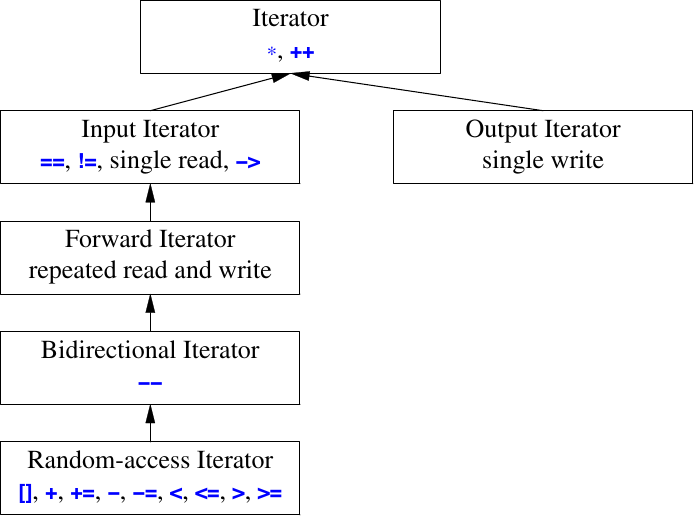
\includegraphics[height=0.8\textheight]{img/iterators.png}
\end{frame}

\begin{frame}[fragile]
  \frametitle{Does our iterator work?}
\lstset{language=C++,
                basicstyle=\ttfamily,
                keywordstyle=\color{blue}\ttfamily,
                stringstyle=\color{red}\ttfamily,
                commentstyle=\color{green}\ttfamily,
                morecomment=[l][\color{magenta}]{\#}
}
\begin{lstlisting}
  template <typename T>
  class List<T>::Iterator {
    ...
  };
\end{lstlisting}
\end{frame}

\begin{frame}[fragile]
  \frametitle{Does our iterator work?}
\lstset{language=C++,
                basicstyle=\ttfamily,
                keywordstyle=\color{blue}\ttfamily,
                stringstyle=\color{red}\ttfamily,
                commentstyle=\color{green}\ttfamily,
                morecomment=[l][\color{magenta}]{\#}
}
\begin{lstlisting}
  #include <iterator>

  ...
  
  template <typename T>
  class List<T>::Iterator : public
    std::iterator<std::forward_iterator_tag, T> {
    ...
  };
\end{lstlisting}
\end{frame}

\begin{frame}[fragile]
\lstset{language=C++,
                basicstyle=\ttfamily,
                keywordstyle=\color{blue}\ttfamily,
                stringstyle=\color{red}\ttfamily,
                commentstyle=\color{green}\ttfamily,
                morecomment=[l][\color{magenta}]{\#}
}
\begin{lstlisting}
  template <typename Cat,
            typename T,
            typename Dist = ptrdiff_t,
            typename Ptr = T*,
            typename Ref = T&>
  struct iterator{
    using value_type = T;
    using difference_type = Dist;
    using pointer = Ptr;
    using reference = Ref;
    using iterator_category = Cat;
  };
\end{lstlisting}
\end{frame}
